
%(BEGIN_QUESTION)
% Copyright 2013, Tony R. Kuphaldt, released under the Creative Commons Attribution License (v 1.0)
% This means you may do almost anything with this work of mine, so long as you give me proper credit

Suppose two identical pumps exhibit the exact same pump curve shown below:

$$\includegraphics[width=15.5cm]{i03560x01.eps}$$

If these two pumps are connected in {\it series} with a suction pressure of 45 PSI ($P_1$ = 45 PSI), calculate pressures $P_2$ and $P_3$ as well as total discharge flow rate when the flow rate through each pump is 150 GPM:

$$\includegraphics[width=15.5cm]{i03560x02.eps}$$

\filbreak

If these two pumps are connected in {\it parallel} with a suction pressure of 45 PSI ($P_1$ = 45 PSI), calculate pressures $P_2$ and $P_3$ as well as total discharge flow rate when the flow rate through each pump is 150 GPM:

$$\includegraphics[width=15.5cm]{i03560x03.eps}$$

\vskip 20pt \vbox{\hrule \hbox{\strut \vrule{} {\bf Suggestions for Socratic discussion} \vrule} \hrule}

\begin{itemize}
\item{} Explain how series and parallel pumps act much the same as series and parallel {\it electrical} sources.
\item{} Where might an engineer choose to use series pumps versus parallel pumps in a piping system?
\end{itemize}

\underbar{file i03560}
%(END_QUESTION)





%(BEGIN_ANSWER)

According to the pump curve, the pressure will be 60 PSI at a flow rate of 150 GPM.  This means each pump boosts its suction pressure by 60 PSI at the discharge.  

\vskip 10pt

In the series configuration, this means $P_2 = P_1 + 60$ and $P_3 = P_2 + 60$.  Therefore, $P_2$ = 105 PSI and $P_3$ = 165 PSI.  Total flow will be 150 GPM.

\vskip 10pt

In the parallel configuration, this means $P_2 = P_1 + 60$ and $P_3 = P_1 + 60$.  Therefore, $P_2$ = $P_3$ = 105 PSI.  Total flow will be 300 GPM.

%(END_ANSWER)





%(BEGIN_NOTES)


%INDEX% Final Control Elements, pump: pressure/flow curve

%(END_NOTES)


